\documentclass[8pt,a4paper]{article}
\usepackage{clrscode}
\usepackage[conEntregas]{caratulaTP1}
\usepackage[spanish]{babel} % para que comandos como \today den el resultado en castellano
\usepackage{a4wide} % márgenes un poco más anchos que lo usual
\usepackage[T1]{fontenc}
\usepackage{textcomp}
\usepackage{graphicx}
\usepackage{enumitem}
\newcommand{\subscript}[2]{$#1 _ #2$}
\usepackage[utf8]{inputenc} 
\usepackage{pdfpages}
\usepackage{amsmath}
\usepackage{vmargin}
\setpapersize{A4}
\setmargins{0.5cm}       % margen izquierdo
{0.5cm}                        % margen superior
{19.0cm}                      % anchura del texto
{26.42cm}                    % altura del texto
{3pt}                           % altura de los encabezados
{1cm}                           % espacio entre el texto y los encabezados
{0pt}                             % altura del pie de página
{1cm}                           % espacio entre el texto y el pie de página
\usepackage{ftnxtra}
\usepackage{listings}
\usepackage{xcolor}
\lstset { %
    language=C++,
    backgroundcolor=\color{black!5}, % set backgroundcolor
    basicstyle=\tiny,% basic font setting
    breaklines=true,
}

\begin{document}
\titulo{Trabajo Práctico 1}
\subtitulo{Eligiendo justito}

\fecha{\today}

\materia{Algoritmos y Estructura de Datos III}

\integrante{Buceta, Diego}{001/17}{diegobuceta35@gmail.com}
% Pongan cuantos integrantes quieran

\maketitle

\newpage
%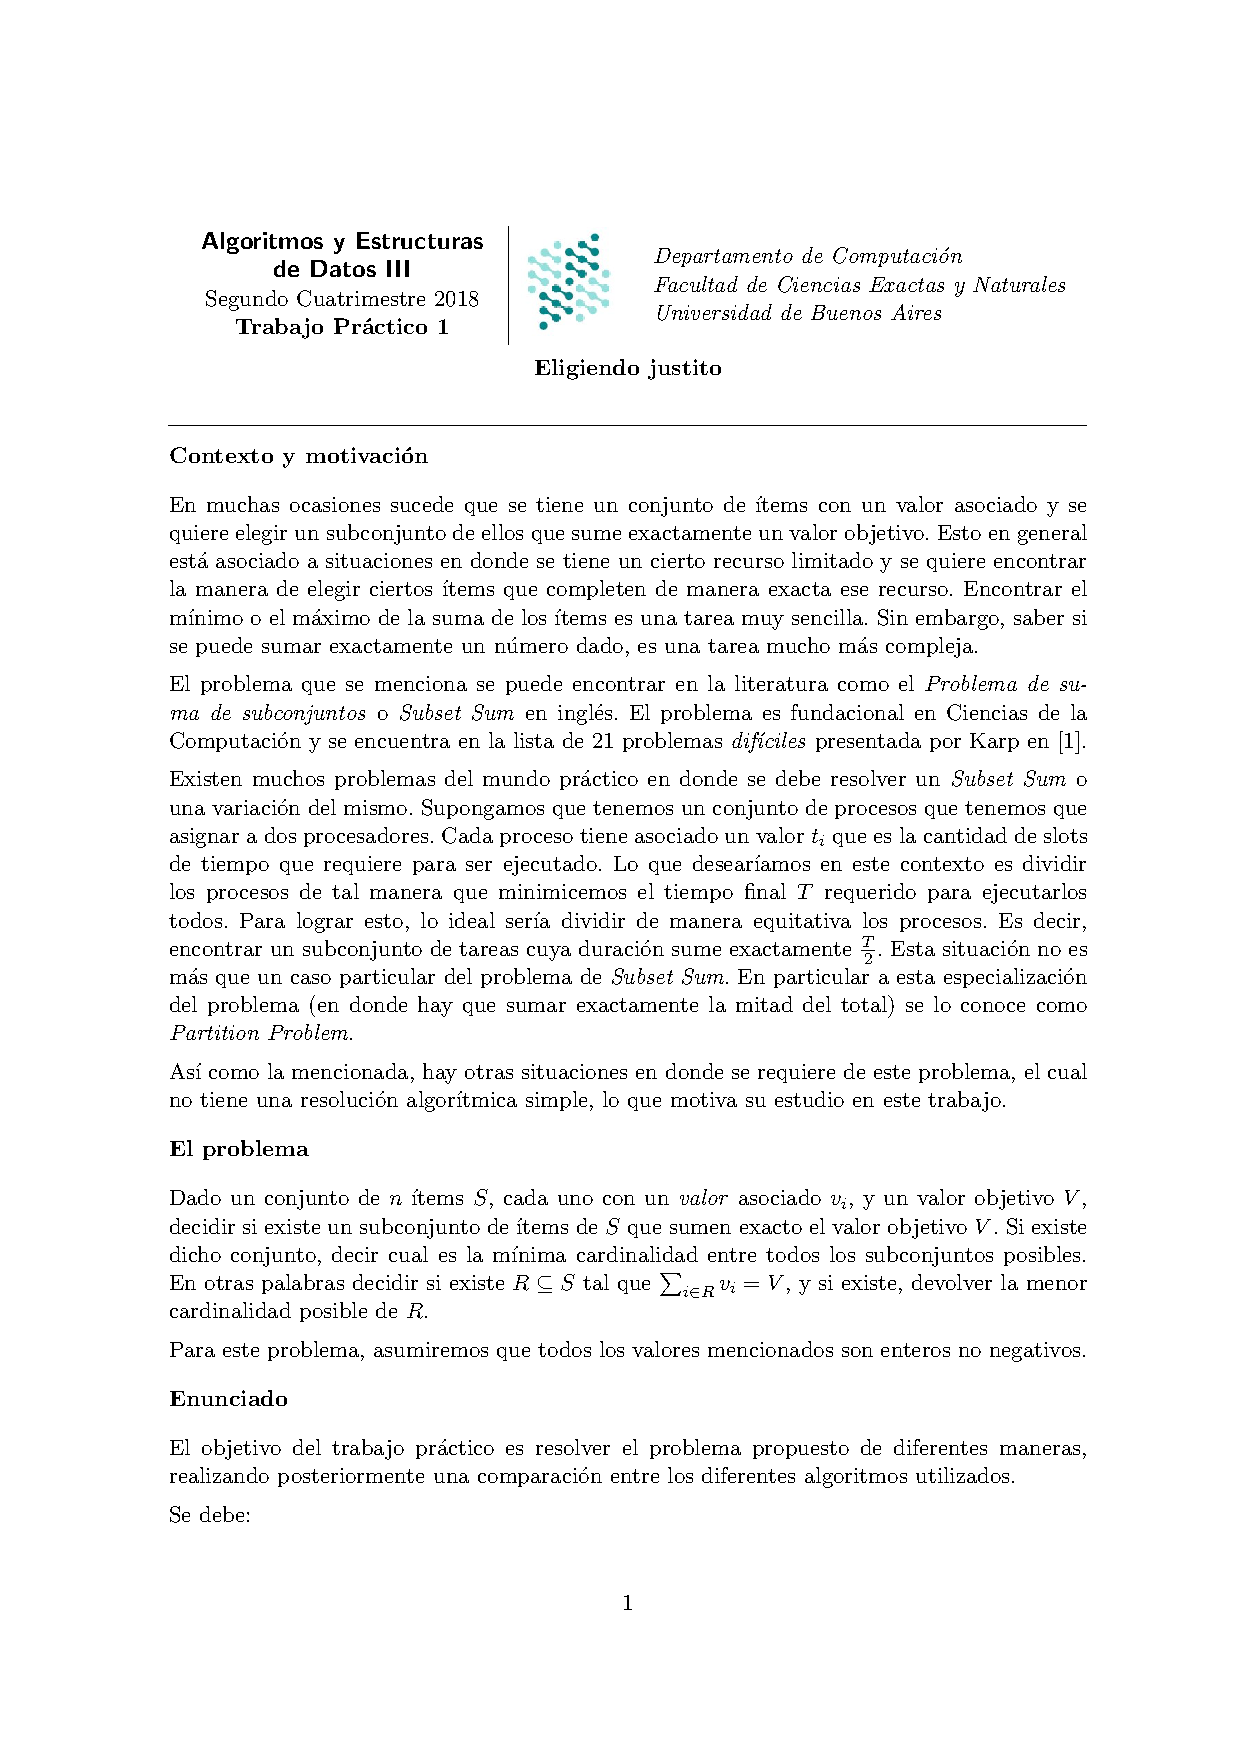
\includepdf[pages={1,2}]{tp1.pdf}

\section{Introducción}
\subsection{El problema y sus análisis}
\begin{verse}
	El subset sum problem o problema de la suma de conjunto es un problema muy conocido dentro de las ciencias de la computación y matemática por ser un objeto de estudio dentro de la clase  NP-problem \footnote{Problemas de decisión y optimización donde se busca encontrar si existe solución o si existe una mejor que la conocida}, se destaca por su facilidad para describirlo y gran dificultad para resolverlo. Los algoritmos más conocidos que pueden resolverlo tienen una complejidad temporal exponencial y esto se traduce en imposibilidad de resolverlo en casos donde la cantidad de elementos sea grande. \\
Además de las diferentes versiones de este problema \footnote{Problema de la carga de la mochila; Problema de selección de conjuntos de un conjunto, etc} existen usos muy diversificados en el ámbito cotidiano y científico. No solo sirve como fuente de nuevas investigaciones en el campo de la teoría de complejidad sino también en ramas como la criptografía, programación genética, etc$[3][4]$. Imaginemos un algoritmo que resuelva problemas a modo de entrenamiento, problemas de tamaños variados y que en muchos casos es necesario clasificar las diferentes soluciones. En los algoritmos genéticos se suele desarrollar un algoritmo que funcione o se comporte como un gen y evaluarlo en consecuencia. Existen casos en los que el output no tienen una correlación real con un gen y es necesario técnicas de apartado o filtrado obtener los más aproximados, y una de ellas está fuertemente relacionada con el Subset Sum Problem.

\bigskip
	Definición: Dado C conjunto de enteros no negativos y V entero no negativo se desea saber si existe un s $\subseteq$ S tal que $\sum_{r \in R}r$ = V, y si existe que tenga la mínima cardinalidad.
	
	\paragraph{Intuición} 	Una de las primeras aproximaciones para buscar una solución puede ser la de formar todos los conjuntos posibles con los elementos de S y analizar si alguno suma V. Por un lado, este algoritmo asegura que si existe solución se va a encontrar; por el otro lado y como contrapartida de lo anterior, si no existe solución o S es muy grande la cantidad de pruebas que son necesarias superará las capacidades de cómputo actuales. En la actualidad hay diversas ramas que se encuentran con estas dificultades, y la manera en que se suelen evitar es utilizando aproximaciones para el problema y no algoritmos exactos$[5]$. reducir esto tampoco tiene sentido la suposición de determinadas características de S, como el orden de sus elementos, dado que siempre se verificarán todos los subconjuntos.
	%Un tamaño de S mayor a 80 con este tipo de técnicas significaría un desafío para las capacidades de los procesadores actuales. Si bien las instrucciones por segundo que pueden realizar dependen de muchos factores como cantidad de instrucciones por ciclo del reloj de procesador, cómo interactúa un determinada software con el procesador, la memoria, núcleos del procesador, factores externos, etc, solo un vistazo a la siguiente tabla evidencia aún más el problema. 	\bigskip
		 %El problema crece exponencialmente respecto al crecimiento de S y si se tiene en cuenta que las procesadores de computadoras personales en promedio pueden tener alrededor de 700GFlops \footnote{Billión de operaciones flotantes por segundo, medida que se utiliza para medir perfomances en los campos científicos computación}, lo que establece una proporción aproximada entre los calcúlos de cantidad de subconjuntos y capacidad de operaciones del procesador de 1 $\approx$ 2000000 operaciones.	\bigskip
	
%\begin{center}
%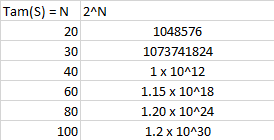
\includegraphics[scale=.7]{tabla.png}
%\end{center}
	\paragraph{Otras formas} Los análisis previos arrojan suficientes razones como para ahondar en otras soluciones.
	\bigskip
	
		Una algoritmo publicado por Horowitz Ellis y Sahni Sartaj $[6][7]$ consiste en dividir los n elementos en dos conjuntos separados, cada uno con $\frac{n}{2}$ elementos. Para cada uno de los conjuntos se almacenan en dos listas la suma de los posibles subconjuntos junto con su cardinal. Posteriormente se utiliza algún algoritmo de comparaciones para ordenarlas, L$_{1}$ en orden decreciente y L$_{2}$ creciente, lo que suma una complejidad temporal de 2 $\cdot$ O($2^{\frac{n}{2}} \cdot \frac{n}{2}$). Con las dos listas ordenadas, la idea principal es tomar un elemento de cada lista y compararlo con V. Por un lado se toma el elemento más grande (primero )de L$_{1}$ y el más chico (primero )de L$_{2}$. Entonces: 

	\begin{itemize}
	\item Si la suma supera a V: El algoritmo avanza un elemento en L$_{1}$
	\item Si la suma es menor a V: El algoritmo avanza un elementom en L$_{2}$
	\item Si la suma coincide con V: se muestra la solución.
	\end{itemize}
	%La complejidad temporal sería del orden O($2^{\frac{n}{2}} \cdot n $). Si se tiene en cuenta el crecimiento exponencial reltivo a n, conseguir una solución que reduzca n a $\frac{n}{2}$ no es poca cosa. \\
	
	
%	Otras soluciones proponen encontrar algoritmos pseudo-polinomiales respecto de n en complejidad temporal. Dado que se busca responder a un problema de forma exacta, las complejidades polinomiales no se pueden esperar.
%	A modo de esclarecer, establezcamos qué es uno y otro.\footnote{Definiciones tomadas del libro Thomas Cormen, Introduction Algorithms. Capítulo NP-Problems, página 1048.}
%	Por un lado, la complejidad de diferentes algoritmos puede cambiar radicalmente en función de los parámetros que depende, y en diferentes circustancias o bajo determinadas suposiciones pueden tomarse los que se consideren apropiados.\\
%	Por ejemplo, en un algoritmo de ordenamiento de comparacion1es, la mejor complejidad que se puede tomar es O($log_2 n \cdot n$), con n cantidad de números. Sin embargo, si se sabe que los números están acotados por una constante K, podría aplicarse un counting-sort y reducir la complejidad a O(K + n) $\approx $ O(n). En caso de que k esté acotado por n, el algoritmo sería O(2n), o sea lineal.\\
%	Este análisis permite ver que incluso definiendo la complejidad en función del tamaño de la entrada los resultados pueden varían. \\
%	La definición formal de complejidad algorítmica temporal habla de que se mide en función del tiempo requerido en función del tamaño de la entrada.
%	Trabajando con enteros de una cantidad acotada de k bits, podemos establecer que la complejidad de nuestra entrada sería O(k $\cdot$ n) $\approx$ O(n).\\
%	\subparagraph{Definición:}	
%	Un problema tiene complejidad en tiempo polinomial si existe un algoritmo que lo resuelva en O($n^{m}$), donde m es constante. Si el problema se puede resolver se lo denomina fácil o tratable y en caso contrario difícil o no tratable. Imaginar esto no resulta complicado dado que m podría ser un número grande como 100 para un exponente y si bien $2^{100}$ sigue siendo polinomial la realidad es que ahora sería un problema difícil. \\ Por esto, existen muchas consideraciones para las complejidades dentro de lo polinomial: pseudopolinomial, quasipolinomial, subpolinomial, etc, pero sólo vamos a adentrarnos en un caso más para nuestro análisis.\\
%	Cuando se habla de algoritmo pseudo-polimial significa que es polinomial respecto del máximo valor númerico de la entrada, y no del tamaño de la entrada.
%	O sea que si podríamos suponer que existe una cota para los valores de S, digamos que están acotados por k = $n^{2}$ y hay n = 100, entonces ninguno superará a 10000. Entonces el algoritmo sería polinomial en esa cantidad fija, digamos W y como es acotada por un polinomio de n, digamos $n^{m}$ entonces el algoritmo es polinomial O($n^{m \cdot W}$).

%Un breve análisis de este problema permitió profundizar acerca de las soluciones encontradas hasta el momento, las diferentes técnicas y formas de expresar sus dificultades utilizadas, y por qué es un objeto tan importante dentro de las ciencias de la matemática y computación este tipo de problemas considerados los NP-P problems.
\end{verse}
\section{Algoritos presentados}
En este trabajo presentaremos diferentes algoritmos con los que buscaremos experimentar y encontrar los contextos en los cuales sería beneficioso la aplicación de alguno de ellos.
\subsection{Fuerza Bruta}
Esta forma de resolver el problema está fuertemente relacionada con las primeras técnicas que surgieron para el problema de la suma de subconjuntos. Lo primero que debe hacerse es definir un dominio de posibles soluciones del problema, y posteriormente describir un algoritmo que permita alcanzarlas a todas. \\

	En nuestro problema, vamos a definir nuestro espectro de posibles soluciones al conjunto de partes del conjunto inicial, S. Este conjunto estará formado por todos los posibles subconjuntos que se puedan tomar con elementos de S. Dado que cada elemento tiene dos opciones, estar o no en un determinado subconjunto, las opciones entonces son: 2 $\cdot$ 2 $\cdot$ 2  $\cdots$ 2 = $2^{n}$
%Por la propia definición, es trivial que si llegará a existir un conjunto R contenido en S y que la sumatoria de sus elementos sea V lo vamos a poder encontrar. Además, almacenando como nueva solución sí y solo sí la encontrada es mejor que la anterior o si no existía,se encontraría en particular la que tenga menos elementos.
\subsection{Algoritmo}

% Updates to \Then and \Else
\renewcommand{\Then}{%
  \textbf{then}\stepcounter{indent} }
\renewcommand{\Else}{%
  \kill\addtocounter{indent}{-1}%
  \liprint\textbf{else}\>\>\stepcounter{indent}}
\renewcommand{\Until}{%
  \addtocounter{indent}{-1}%
  \kill\liprint\textbf{until} }

\begin{codebox}
  \Procname{$\proc{FuerzaBruta}(Conjunto(enteros):C,entero: V)$}
  \li $i \gets 0$
  \li $P \gets generarPartes(C)$
  \li $sol \gets -1$
  \li $n \gets Tam(C)$
  \li \Repeat
  \li   $suma \gets sumaElementos(P, i)$
  \li   $card \gets cantElementos(P, i)$
  \li   \If $suma == V$ \Then
  \li 	\If $sol == -1$ \Then
  \li     $sol \gets card$
  \li 	\Else 
  \li 	\If $sol > card$ \Then
  \li 	$sol \gets card$
  		\End
        \End
        \End
  \li \Until $i <= 2^{n}$
\end{codebox}

%\paragraph{Detalle}

%	El algoritmo se basa en analizar la suma de elementos de cada uno de los $2^{n}$ subconjuntos que puede formarse y compararlos con V. Si ya existiese una solución sólo la renombraríamos si la actual es mejor, es decir, el subconjunto tiene menos elementos.
%	\\ Los puntos importantes del pseudocódigo están en (2)(6)(7) porque es donde están los pasos {\it no triviales}. \\
\subparagraph{Función: generarPartes} El código fuente del problema genera el conjunto de partes de la siguiente manera: una variable $i$ se mueve entre 0 y $2^{n}$ - 1, y en cada uno de esos valores analiza su representación en bits y además otra variable $j$ se mueve entre 0 y n-1. Es decir, cada vez que i actualiza su valor, j se actualiza n veces. En esas n comparaciones lo que se hace es analizar si el bit jésimo se corresponde un bit marcado en uno de i. Si esto pasa, significa que en el subconjunto iésimo debe estar el elemento j, y así para cada elemento. Esto se hace mediante el corrimiento de bits en O(1) que ofrece $C++$.
\subparagraph{Función: sumaElementos y cantElementos} Dado un conjunto de conjuntos y un valor,  una retorna la suma y la otra el cardinal del subconjunto i-ésimo. A modo de una mejor visualización de las ideas del algoritmo estas funciones cumplen un objetivo simbólico y no tienen una correspondencia simétrica con el código, en caso de plasmar este pseudocódigo en un lenguaje, simplemente cambiará la complejidad espacial debido a que habría $2^{n}$ subconjuntos almacenados.

\subsubsection{Complejidad}
Desde el punto de vista de complejidad, si se define en función del tamaño de entrada, y tomando n como el tamaño de S, nuestro algoritmo será $\theta$(n $\cdot$ 2$^{n}$), porque se recorrerá cada subconjunto del conjunto de partes de S y para cada uno revisará cuáles de los n elementos de S están en ese subconjunto.\\
%Si se definiera en función de m = $\max C$ y si m = $2^{n}$, la complejidad seria O(m $\cdot \log_{2}{m}$ ), valor que en la práctica se podría considerar lineal (respecto a m), una diferencia demasiado grande con respecto a una complejidad exponencial. Resulta interesante pensar en cómo se verá todo estas variaciones en las experimentaciones de este algoritmo.

\subsection{Backtracking}
Lo que caracteriza a esta forma de resolver el problema es que vamos a buscar definir situaciones en las que seguir computando la solución no tenga sentido. Esto quiere decir abandonando posibles candidatos a solución por temás de optimalidad o posibilidad de la solución, a esto se lo denomina podas. \\
%Si se modela el Backtracking como un árbol binario[\footnote{Donald Knuth. \it{The Art Of Computer Programming : Fundamentals Algorithms.} Capítulo 2}] puede pensarse que cada nodo representa un nuevo sub-problema o llamada recursiva del problema anterior y puede tener a lo sumo dos llamadas recursivas, es decir, dos hijos. Esto significa que en un árbol balanceado la profundidad será $\log_{2}(2^{n})$ = $n$ y las llamadas recursivas va a estar acotada superiormente por la cantidad de nodo que será:$\approx$ $2^{n}$

%Para nuestro caso en particular, vamos a suponer que nuestro conjunto C viene ordenado. Podemos hacerlo porque en caso de que no venga se lo ordena en $\log_{2}n \cdot n$ con algún algoritmo que como merge-sort, que no afecta la complejidad a la que nos debemos ajustar. La razón de tenerlo ordenado en forma creciente es que vamos a poder establecer cotas de complejidad más fuertes.
\subsubsection{Podas}
\begin{itemize}
	\item 
	Por optimalidad: Si en el proceso de computo de una posible solución, se llegara al caso en que el subconjunto de elementos actual contiene más elementos que la mejor solución encontrada hasta ahora, entonces no se buscará y computará ninguno de los subconjuntos que surjan de tener como los primeros k elementos del subconjunto actual y siendo k el tamaño de éste.
	\item 
	Por factibilidad: Si en el proceso de cómputo de una posible solución, se llegara al caso en que la sumatoria de los elementos del conjunto formado actual supera a V, significa que no tiene sentido probar con a ninguno de los elementos hacia la derecha, porque están ordenados de forma creciente, y ninguno de los conjuntos que surjan de combinar los elementos restantes de S con el conjunto actual van a funcionar.
\end{itemize}

%Breve ejemplo con C = $\{$ 2, 3 , 6$\}$ y valor objetivo V = 5.\\
%Se observan los nodos verdes que son los caminos que se siguen y los rojos los que se podarían
%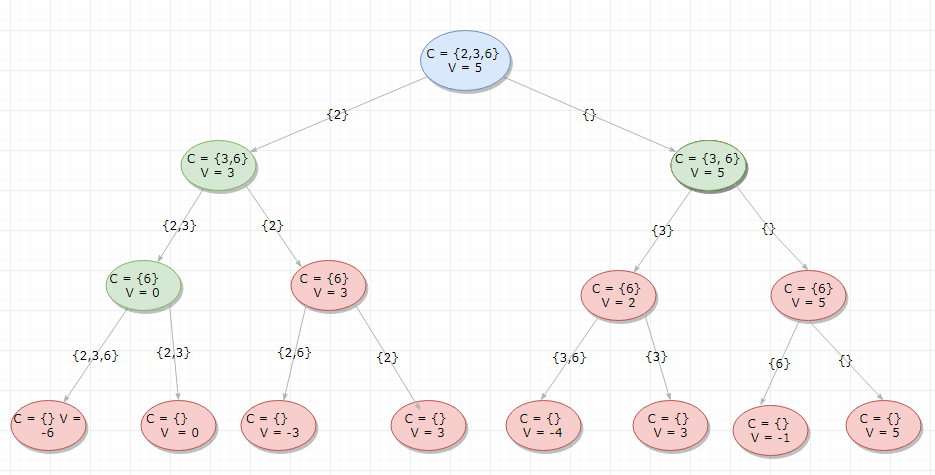
\includegraphics[scale=.7]{grafico_backtracking.png}

La siguiente imagen muestra la idea de las podas. Si tomamos el punto amarillo superior como el inicio de una parte de los posibles caminos del problema total vemos cómo las flechas verdes marcan los caminos que se siguieron por cada nodo y cómo al llegar a puntos \textcolor{red}{problemáticos} las flechas rojas marcan el retroceso y recorrido de otro camino, hasta agotarlos a todos. Los puntos \textcolor{red}{problemáticos} simbolizan otros inicios de conjuntos de caminos que por algún motivo se decide 'podarlos' y no analizarlos en profundidad.

\begin{center}
\includegraphics[scale=.2]{backtrack}
\footnote{Imagen tomada del blog de Steve Pemberton}
\end{center}
\subsubsection{Algoritmo}



\begin{codebox}
  \Procname{$\proc{Backtracking}(Conjunto(enteros):C,entero: V)$}
  \li $sol \gets -1$ \li 
  \If $V$ $=$ $0$ \Then \li 
  	$sol \gets 0 $ \li 
  	$Devolver$ $0$
  \End 
  \li $OrdenarAsc(c)$
  \li $sol \gets auxBacktracking(c,0,V,sol,0,0)$
\li \If $sol$ = $-1$ $or$ $sol$ > $|C|$ \Then
\li 	$Devolver -1$\li 
\Else \li 
		$Devolver$ $sol$
	\End
  	\End
\end{codebox}

\begin{codebox}
  \Procname{$\proc{auxBacktracking}(Conjunto(enteros):C,entero:sol,entero: V, entero:desde,entero:sumaElem,entero:cantElem)$}
\li 	\If $sumaActual$ > $valorObjetivo$ \Then 
		\li $Devolver$ $|C|+1$ 
		\End
	\li \If $sol!=-1$ $and$ $cantElem$ >= $sol$ \Then
		\li $Devolver$ $|C|+1$
  		\End
  	\li \If $sumaActual$ $=$ $valorObjetivo$ \Then
  	\li $sol \gets cantElem$
  	\li $Devolver$ $0$ 
  	\End
  	
  	\li \If $desde$ $<$ $|C|$ \Then
  	\li \If $c[desde]$ $+$ $sumaActual$ > $valorObjetivo$ \Then
  	\li $Devolver$ $|C|+1$ \li
  	\Else \li$valor1 \gets auxBackTracking(c,desde+1,valorObjetivo,sol,sumaActual,cantElem)$
  	\li $valor2 \gets 1+auxBacktracking(c,desde+1,valorObjetivo,sol,sumaActual+c[desde],cantElem+1)$
  	\li $Devolver$ $min(valor1,valor2)$
  	\End
\end{codebox}

\subparagraph{Detalle} 

\begin{verse}
La función principal es Backtracking, que se encarga de recibir el conjunto con el que trabajar, el valor objetivo, y prepara lo necesario para resolver el problema con metodología de Backtracking. En nuestro caso, ordena el conjunto, según documentación de C++, en O($ n \cdot \log{n})$ e inicializa los flags que usará la función recursiva. Estos son: sumaActual, que contiene la suma de los elementos tomados como posible solución por una determinada rama; cantElem que contiene la cantidad de elementos tomados como posible solución por una determinada rama; desde, que permite que cada llamado recursivo sepa desde donde a agregar elementos a la solución en una determinada rama; sol, que es donde se almacena la mejor solución actual que se encontró para el problema y que cada llamado recursivo revisa para conocer si es posible que esa rama mejore la solución actual y en caso contrario podarla. Esta variable, al igual que los conjuntos, se utilizan mediante referencias para no hacer copias de C que puede ser excesivamente grande y para poder conocer en cada subproblema la solución encontrada actualmente, que pudo haber sido actualizada por una rama posterior a la que generó este llamado recursivo y de esta forma puede tener acceso a la solución actual.
\end{verse}

\subsubsection{Complejidad}

Respecto a la complejidad temporal y estableciéndola en función de tamaño de la entrada, $|$S$|$ = n, veamos que el peor caso sería si para ningún llamado recursivo existe poda, es decir, el valor objetivo es mayor que cualquier sumatoria de subconjunto de C (no hay poda de factibilidad) y como tampoco se encuentra solución alguna no se puede podar llamados recursivos por poda de optimalidad. De modo que terminaría después de probar con cada subconjunto (el conjunto de partes de C).\\
Cada elemento de C (n en total), generaría dos llamados recursivos con el flag desde = desde + 1, o sea que estos llamados recursivos del elemento $C_{1}$ generarían a su vez cada uno de ellos otros dos llamados, pero de tamaño |C|-1 el conjunto y así sucesivamente. Esto generaría un árbol binario completo de $2^n$ nodos y n hojas. Como cada llamado recursivo va actualizando la suma de los elementos que le llega de su predecesor, no aporta a la complejidad (más alla de los $2^{n}$ nodos que se recorren) la suma de los elementos que se consideran en esa rama de soluciones. La complejidad quedaría entonces O($2^{n}$) + O(n $\cdot$ $\log{n}$) = O($2^{n} + (n \cdot \log{n})$) $\in$ O$(2^{n}$ $\cdot$ $n)$.



\subsection{Programación Dinámica}

Esta técnica se basa en utilizar la metodología de {\it divide and conquer \footnote{Metodología que busca simplificar un problema grande o complicado en problemas más chicos y simples de una forma recursiva}} y almacenar los resultados calculados para no tener que volver a hacerlo cuando se repita un problema. Para poder aplicar usar programación dinámica es necesario que se cumpla entonces: 
\begin{itemize}
	\item
	El problema pueda ser dividido en subproblemas y que la solución que se encuentre para cada uno de ellos sea óptima, para así construir la solución del problema inicial de forma óptima \footnote{Este concepto suele denominarse como: {\it principio del óptimo}}
	
	\item 	
	Los subproblemas compartan soluciones\footnote{Se denomina a esto subproblemas superpuestos y un ejemplo muy conocido es la sucesión de Fibonacci}, si no no tendría sentido almacenar las soluciones.
\end{itemize}


\begin{center}
En este gráfico se puede ver cómo los nodos que ya se calcularon están en azul y los rojos serían nodos que no se calculan porque ya se obtuvo la información que le corresponde.
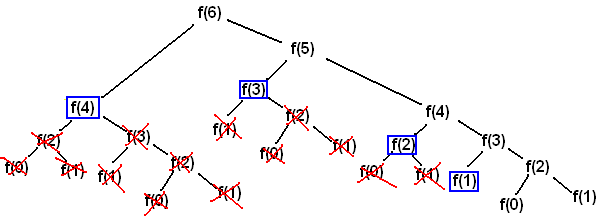
\includegraphics[scale=.4]{fibonacci_pd.png}
\end{center}

Dentro de este tipo de programación hay varios  algoritmos de implementación. Uno es el de top-down (por el significado en ingles de de arriba para abajo) o memoización y el otro bottom-up (por el significado en ingles de abajo hacia arriba), aunque existen bibliografías que consideran sólo a top-down como programación dinámica.
\\
En este análisis se implementarán de ambas formas de forma que se pueda ahondar más acerca de los beneficios de ambos. 
\bigskip
\subsubsection{Análisis}
\begin{verse}
La idea de un algoritmo que implemente {\it divide and conquer} y almacenamiento de subproblemas, sugiere empezar pensando este problema y dividiéndolo en problemas pequeños.\\
Se puede afirmar que la solución, si existe, puede dividirse en dos casos: la solución no contiene al primer elemento de C y entonces la solución resulte de formar V con la mínima cantidad de elementos de C': 
\[ C' = C - \{e_{1}\}\]
Y en particular debe ser óptima. Supongamos por el absurdo que no. La solución al problema sería K $\leq$ |C'|. Supongamos que existe un Q < K que es solución. Pero esto no puede pasar, porque por la propia definición de nuestra solución, se va a devolver la mínima cantidad de elementos, entonces no puede existir un valor menor de elementos que sea solución.
\\
La otra posible solución sería que $e_{1}$ sí sea parte de la solución, es decir, habría que encontrar elementos que sumen V' con los elementos del conjunto C' :
 \[ C' = C - \{e_{1}\}\]
\[ V' = V - e_{1}\]
O sea que la solución óptima sería 1 + K, K $\leq $ |C'|, K solución. Si existiese un Q $ $ < $ $1+K y la suma de los elementos de Q = V', es decir hay una solución mejor para el problema con C' y V'. Pero entonces ahora K $=$ Q y la solución óptima es K + 1, donde el 1 representaría el primer $e_{1}$ que por el análisis de este caso formaba parte de la solución óptima.
\end{verse}

\bigskip
\subsubsection{Formulación recursiva}
Se define PD una función que recibe un conjunto S, de elementos enteros no negativos, un valor V entero no negativo y un entero que representa el tamaño de S inicial, devuelve el mínimo cardinal del subconjunto s perteneciente a S que todos los elementos suman V; si no existe se devuelve n+1, n tamaño de S, simbolizando la imposibilidad de encontrar solución. \\
\[
\begin{array}{@{} r @{} c @{} l @{} }
&PD(S, V, n)&{}=\displaystyle
\begin{cases}
\ n+1 &\text{si } \text |S| = 0 \wedge V \neq 0 
\\
\ 0 &\text{si } \text V = 0 
\\
PD($\{$e_{2},e_{3},\dots,e_{n}$\}$,V,n)  &\text{si } e_{1} $>$ V
\\
1 &\text{si } e_{1} = V
\\
\min_{} (1 + PD($\{$e_{2},e_{3},\dots,e_{n}$\}$, V - e_{1}, n),PD($\{$e_{2},e_{3},\dots,e_{n}$\}$, V, ))&\text{otro caso }
\\
\end{cases}
\end{array}
\]
Cabe resaltar que a modo de una formulación más intuitiva, cada llamado se hace envíando un S modificado, algo que en una implementación tendría un costo muy grande de copias, es por eso que en código se utilizará una referencia (nunca se copia) al conjunto inicial (y no se modificará) y para saber los límites del conjunto en el llamado recursivo actual se usa un flag {\it desde} que hace referencia a los elementos que se pueden usar en ese llamado.
\subsubsection{Algoritmo Top Down}
\begin{codebox}
\Procname{$\proc{AUX-Topdown}(C,V)$}
  \li \If $|C|$ $=$ $0$ \Then
  \li \If $V$ $=$ $0$ \Then
  	\li $sol \gets 0$
  	\li $Devolver$ $0$
  	\li \Else
  	\li $sol \gets -1$
  	\li $Devolver$ $-1$
  	\End
  \li \ElseIf $V$ $=$ $0$ \Then
  	 \li $sol \gets -1$
  	\li $Devolver$ $-1$
  \End
	\li $soluciones \gets$ $matriz$ $de$ $n$ $X$ $V$ $con$ $-1$ $en$ $los$ $valores$
	\li $soluciones_{0,0} \gets 0$
	\li $sol \gets Topdown(C,V,0,soluciones,|C|)$
	\li \If $sol$ $>$ $|C|$ $or$ $sol$ $=$ $-1$\Then
		\li $Devolver$ $-1$
		\li \Else
		\li $Devolver sol$
	\End

\end{codebox}

\begin{codebox}
\Procname{$\proc{Topdown}(C,V, desde, memoria,n)$}
 \li \If $desde < 0$ \Then
  	\li \If $V =0$ \Then 
  	\li $devolver:0$
  	\li \Else
  	\li $devolver:n+1$
  \End 
 \End
  \li \If $NoExiste(C,V,desde,memoria)$ \Then
 
\li \If $c_{desde}==V$ \Then
	\li	$Guardar(1,V,desde,memoria,n)$
	\li \Else
\li \If $C_{desde} > V$ \Then  
		\li $valor \gets Topdown(C,V,desde-1,memoria,n)$
		\li $Guardar(valor, V, desde, memoria,n)$
		\li \Else
		\li $valor1 \gets 1 + Topdown(C,V-C_{desde},desde-1,memoria,n)$
		\li $valor2 \gets Topdown(C,V,desde-1,memoria,n) $
		\li $valor3 \gets min(valor1,valor2)$ 
		\li $Guardar(valor3,V,desde,memoria,n)$	
  		\End
  \End
  \End
\li $Devolver: -1$  $si$ $memoria_{desde,V} \geq n$
\li $Devolver: memoria_{desde,V}$ $si$ $no$

\end{codebox}

\begin{verse}
Tenemos dos algoritmos, el primero que es el que se encarga de analizar si el problema no es un caso base y devuelve la solución que corresponde y en caso contrario inicializa lo necesario para poder aplicar el algoritmo de Top-Down. Las cosas que se inicializan son, la memoria, implementada sobre una matriz de n x (V+1)\footnote{Se le suma 1 simplemente para tener una columna que se corresponda con el valor objetivo, dado que los indices empiezan en 0 y van hasta tope-1. No modifica la complejidad asintótica esto}, donde se va a reutilizar los subproblemas ya calculados, el flag desde que permite a Top-Down saber desde cuál es el problema actual que hay que empezar a dividir en subproblemas.\\ El algoritmo de Top-Down primero preguntar si ya se calculo previamente el resultado del problema y en caso contrario lo calcula y lo almacena en memoria, que se utiliza mediante referencia para no hacer copias y tenerla todo el tiempo actualizad .\\ Es importante recalcar que tanto Aux-Top-Down como Top-Down utilizan a C por referencia, para no estar haciendo copias, que cuando n es grande podrían significar tiempos de ejecución mucho mayores.
\\
La explicación de complejidad es un poco más difícil que para el próximo algoritmo porque en este hay llamados recursivos que hay que demostrar que no hacen cosas imprevisibles y arruinan la complejidad.\\
Imaginemos a la matriz de n x V, y pensemos que todavía no se calculó ningún resultado. Empezamos de la última fila i y columna j. Puede haber uno o dos llamados recursivos. Si hay uno, necesariamente la posición del proximo subproblema es la de (i-1)(j). Si hay dos,  una de esas posiciones será (i-1)(j)  y la otra (i-1)(j-$C_{k}$), donde k es, en este caso 1, pero que va de 1 a n. La cuestión es que más allá de que se llaman al mismo tiempo, hay un orden. Ese orden permite que cuando se hacen los dos llamados, primero se va a resolver uno y después el otro y si se llegara a dar que el llamado dos cae en una posición de un subproblema que ya calculó el otro llamado, es trivial que la solución se consigue en O(1) en ese llamado y cualquiera que utilice problemas ya calculados por el primer llamado. Si esto lo extendemos a toda la matriz, después del primer o los dos primeros llamados, uno de ellos se va terminar de resolver y recién ahí se resolverá el otro. Y en particular este comportamiento se repite para todos los llamados que generen los llamados del primer llamado (digamos $L{1}$). Como la matriz es finita, para cada fila (n) $L{1}$ va a generar dos llamados como máximo. Cada llamado recursivo se genera porque no había solución para el subproblema. Como la cantidad de subproblemas es n x V y los llamados recursivos se resuelven en orden, la máxima cantidad de llamados tiene que ser n x V, porque si no estaríamos diciendo que se van a hacer llamados recursivos para problemas ya calculados y esto no puede ser porque después de calcularlos los guardamos y particularmente al trabajar por referencia, al actualizar la memoria en un determinado llamado, todos los llamados anteriores que todavía no fueron resueltos tienen la memoria actualizada.
\end{verse}

\subsubsection{Algoritmo Bottom Up}
\begin{codebox}
\Procname{$\proc{BottomUp}(C,V,n)$}
\li $memoria \gets matriz$ $de$ $n$ $\cdot$ $V$ $de$ $enteros$ $vacia$
\li $cargarConValores(memoria,n+1)$
\li $memoria_{0,0} \gets 0$
\li \For $i \gets 2$ \To $n$
\li	 	\For $j \gets 1$ \To $V$
\li 		\If $C_{i} > j$ \Then
\li 			$memoria_{i,j} \gets memoria_{i-1,j}$
\li 	\Else
\li 			$valor1 \gets memoria_{i-1,j}$
\li 			$valor2 \gets 1 + memoria_{i-1,j-c_{j}} $
\li 			$memoria_{i,j} \gets min(valor1,valor2)$ 
		\End	
	\End  
\End
\li $Devolver: -1$  $si$ $memoria_{n,V} \geq n$
\li $Devolver: memoria_{n,V}$ $si$ $no$

\end{codebox}
\begin{verse} 
Inicialmente se inicializa la estructura donde vamos a almacenar los resultados de todos los subproblemas. Particularmente se inicializa la primera fila (la 0) con el valor n+1, que simbolizaría la imposibilidad de formar el valor objetivo con 0 cosas, excepto en la posición 0,0, que la definimos como 0.\\
Esta implementación se corresponde de forma muy evidente con su nombre: si imaginamos un problema como la raíz de un árbol y a los hijos como sus subproblemas es muy intuitivo el funcionamiento. Este algoritmo se basa en empezar resolviendo los subproblemas más chicos y resolver el problema que los generó, es decir, su padre. Dado que el padre de todos es el problema inicial, si repetimos este procedimiento mientras el padre tenga algún predecesor, terminaríamos resolviendo el problema inicial.\\
Como consecuencia de este funcionamiento tan estructurado, se resuelven todos los posibles subproblemas y no los necesarios, como Top-Down, de modo que es esperable que si el tamaño de C o el valor objetivo son grandes, se notará en la performance. Por otro lado la justificación de la complejidad es más simple, dado que no hay llamados recursivos que analizar, sino que se recorren las n x V celdas y se guarda el valor que le corresponde, que viene de alguna celda correspondiente a la fila anterior y alguna columna. Como la primera fila de la matriz tiene los "casos base", cada uno de las n x V iteraciones es O(1) porque simplemente pone en la celda actual el valor de otra celda o el valor del mínimo de otras celdas, que accede en O(1). Entonces es trivial que la complejidad es O(n x V).
\end{verse}


\section{Experimentación}
\begin{verse}
Para la experimentación primero se probará con casos de test para comprobar la correctitud de los algoritmos. Sin embargo y dado que instancias excesivamente grandes demandarían mucho tiempo en hacer el cálculo a mano para comprobar los resultados, se aprovechará la etapa de experimentación con instancias generadas en Python no solo para guardar la información necesaria para la experimentación  sino que también para cada instancia se comparará cada uno de los resultados de los cuatro algoritmos. Evidentemente no es una prueba exacta pero da mayor seguridad a la hora de la correctitud.\\
Las pruebas que se hagan con valores random se harán utilizando la libreria numpy en Python y para el análisis de los resultados de los algoritmos se usará: pandas, seaborn, matplotlib.pyplot y jupyter notebook. Además, se testearán 4 veces cada instancia en cada algoritmo para sacar un promedio de los tiempos de ejecución reduciendo al mínimo los posibles ruidos. Para la ejecución de los algoritmos y sus tiempos se utilizará una porción de código mostrada en una clase de laboratorio de experimentación.
\\
\subsection{Fuerza Bruta y Backtracking: exponenciales}

Los primeros análisis sería interesante empezarlos comparando los algoritmos más básicos como fuerza bruta y backtracking. Posiblemente el algoritmo de fuerza bruta no permita ser computado para tamaños de C excesivamente grandes y los otros algoritmos sí, entonces sería razonable que se experimenten los algoritmos de forma cruzada y estableciendo relaciones y no todos de forma simultánea porque podría perderse información.
Además, la implementación de los algoritmos sugiere que ante contextos de peor caso y |C| razonablemente chico, mientras que para casos de C grandes serían algoritmos sin uso práctico.
\\

\begin{center}
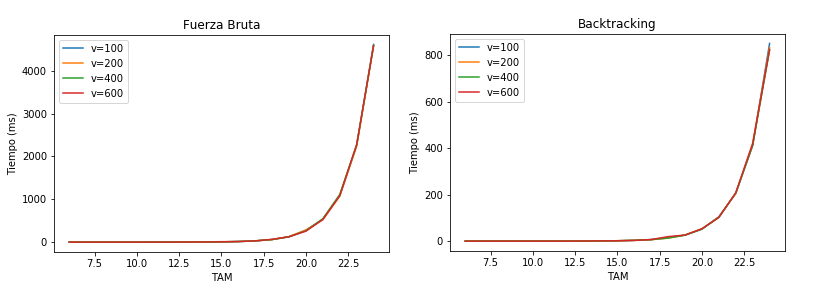
\includegraphics[scale=.7]{bf_var_v_plot.png}
\end{center}
Podemos ver que ambos algoritmos tienen pinta de tener la complejidad exponencial respecto de n anteriormente analizada. Y también se puede inferir que el valor objetivo no es una variable para la complejidad de estos algoritmos, ya que vemos que con diferentes valores objetivos parecen ser iguales crecimientos asintóticos.\\ 
\begin{center}
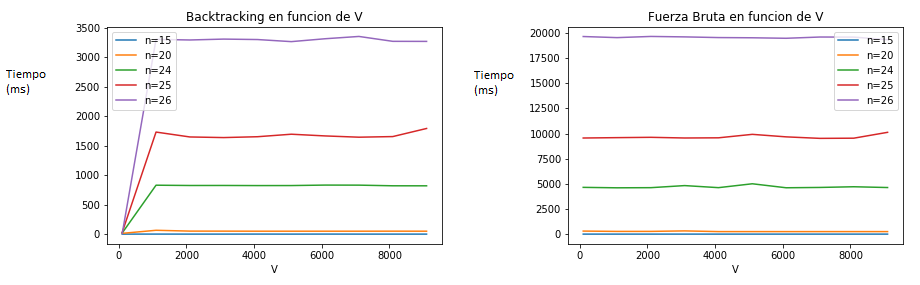
\includegraphics[scale=.7]{bt_bf_var_v.png}
\end{center}
Con estos gráficos podemos confirmar que el valor objetivo no es un factor dentro de la complejidad de estos algoritmos. Podemos ver como a medida que el valor objetivo crece, para n variados en general, los algoritmos son asintóticamente constantes. En Backtracking podemos ver que en los primeros valores de V esto no se cumple, pero es porque en esos valores de V la relación con los elementos de C permite efectuar podas, mientras que para V excesivamente grandes, donde ya no hay podas, el valor de V no afecta. Como conclusión, Fuerza Bruta no es afectada por el valor objetivo, mientras que Backtracking podría tener casos donde la relación de los elementos de C y el valor objetivo permite encontrar una o más soluciones y esto genera podas que en la práctica reduce la complejidad teórica.\\

\begin{center}
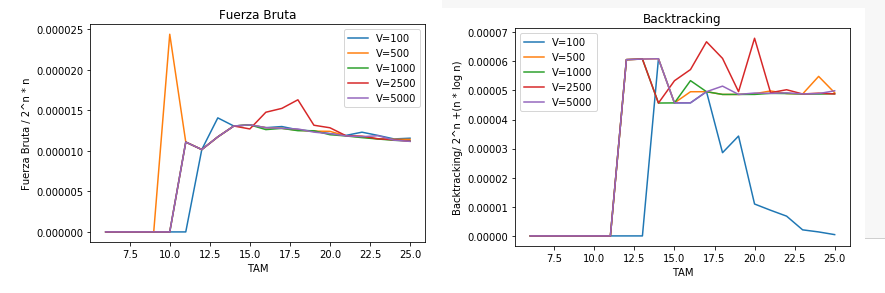
\includegraphics[scale=.8]{btvsbf.png}
\end{center}
Finalmente podemos terminar de afirmar que los algoritmos cumplen con la complejidad teórica, que son efectivamente exponenciales en el peor caso y que las variaciones del valor objetivo no tienen una correlación con la complejidad. El único comentario es que se puede ver como para V $=$ 100 sigue manteniéndose que no constante respecto a la exponencial del backtracking, y eso se debe a como vimos en los anteriores casos, en esos V empieza a encontrar soluciones y funcionar algunas podas y por ello la complejidad es menor. Para los demás casos en donde V es de mucho mayor orden que los elementos de C, backtracking es exponencial (particularmente a la función $2^{n} \cdot n \log{n}$ y fuerza bruta a $2^{n} \cdot n$).\\

\subsection{Top Down y Bottom Up: lineales en n x V}
\begin{verse}
Como antes, comenzaremos analizando con los peores casos y tratando de llegar a ver que cumplen la complejidad anteriormente analizada. En Bottom-Up vimos que siempre resuelve todos los subproblemas en una matriz de n x V, y en Top-Down también existe una matriz de n x V (complejidades espaciales en teoría asintóticamente iguales en ese punto), pero a diferencia sólo resuelve los que necesita, de modo que esperamos ver ciertas diferencias en los mapas de calor.
\end{verse}
\begin{center}
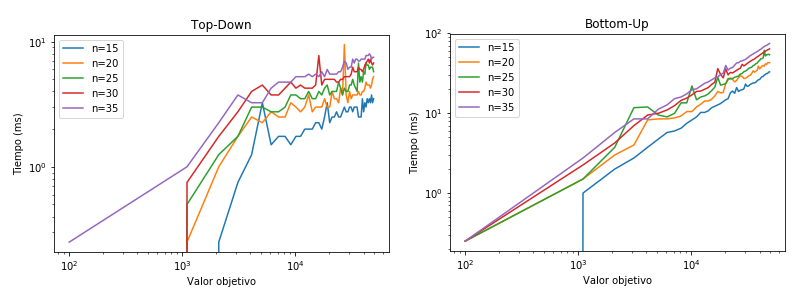
\includegraphics[scale=.9]{tdvsbu_var_n.png}
\end{center}
\begin{verse}
Los gráficos están en escala logarítmica en ambos ejes para una mejor visualización, sobre todo en el eje x donde el valor objetivo va desde 100 a 50000. \\
En ambos podemos inferir que existe un crecimiento dependiente de n y v , porque si bien los algoritmos crecen a medida que aumenta V, también se ve que para C cada vez más grandes el crecimiento también existe. Por otro lado, hay que remarcar que el Top-Down tiene no solo un crecimiento más aplastado, producto de no calcular todos los subproblemas, sino menores tiempos.\\
Veamos los algoritmos en algo que nos permita comparar de forma más clara las variaciones en función de V y n.
\begin{center}
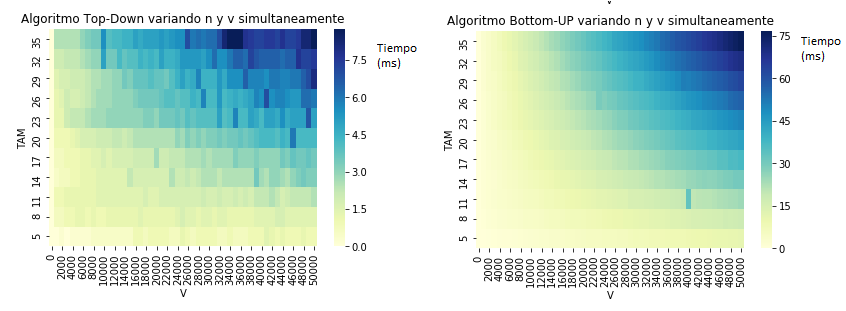
\includegraphics[scale=.8]{tdvsbu_heatmap.png}
\end{center}
Con los mapas de calor se puede observar cómo los aumentos de n y V influyen directo en la performance de los algoritmos de programación dinámica. Sin embargo, también hay que notar que en Top-Down el proceso de aumentar n y V no empeora la performance del algoritmo de forma tan escalonada como en Bottom Up sino que el tipo de instancias definen en parte la performance que tendrá, en función de los subproblemas que tenga que resolver. 
\begin{center}
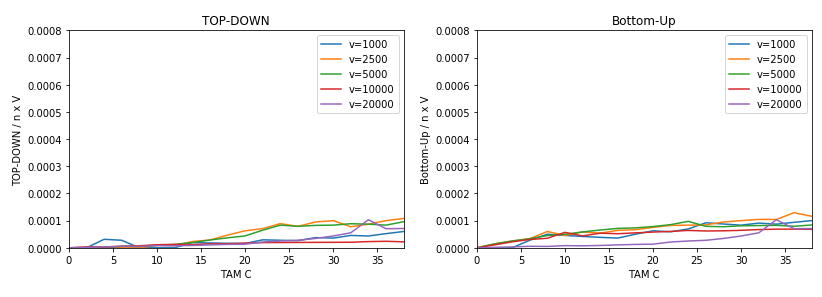
\includegraphics[scale=.8]{td_nxv.png}
\end{center}
De nuevo, con este último podemos terminar de asegurar que los algoritmos tienen la complejidad anteriormente analizada (n $\cdot$ V).
% En los siguientes gráficos vamos a ver un poco más en detalle el comportamiento para V menores, particularmente hasta 1000, que es donde los anteriores no aportaban demasiado.
\end{verse}






\subsection{Backtracking vs programación dinámica}
\begin{verse}
Nota: dado que tanto Top Down y Bottom Up son algoritmos de programación dinámica, vamos a utilizar para los análisis sólo al último como representante de esta metodología.\\
Ahora trataremos de buscar contextos en cada uno de estas metodologías se impongan.\\
Empecemos analizando los mejores casos para Backtracking. Estos necesitan ser instancias en donde se apliquen podas la mayor cantidad de veces posibles, y esto pasa si todo el tiempo se pueden encontrar mejores soluciones o evitamos grandes ramas de soluciones porque los valores de los elementos de C a partir de una posición son mayor que V (y aca ayuda que el Backtracking ordena a C). Fijemos para esto  valores de V entre 0 y $n^{2}$ y los valores de C entre 0 y V, de modo de tener ciertas relaciones entre los valores y que a su vez sean lo suficientemente abarcativos.
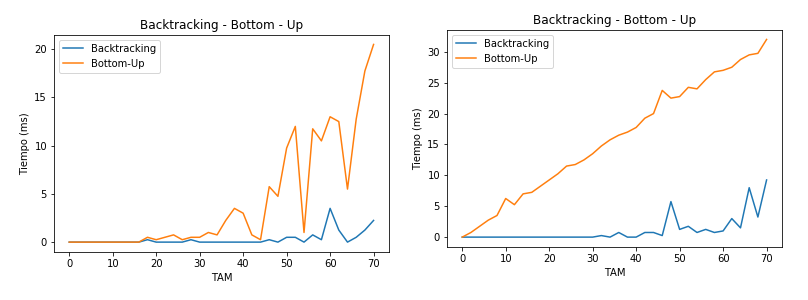
\includegraphics[scale=.8]{buvsbt.png}	
Es apreciable que en este tipo de instancias, la performance de un algoritmo de programación dinámica tiende a ser menor a la de Backtracking, que obtiene muchos beneficios de sus podas. Lo más interesantes es ver (en el segundo gráfico) que si fijamos a V = 10000 (un numero considerablemente grande) y los elementos de C siguen entre 0 y V, el algoritmo de programación dinámica es aún menos eficiente, y es razonable por lo antes analizado, que vimos que depende fuertemente de n y V.\\
Entonces.. cuál serían los casos en donde programación dinámica sea mejor que Backtracking? Bueno por un lado ya sabemos que cualquier instancia en donde los elementos de C son de mucho menor orden que V, Bactracking se comporta exponencialmente, como un algoritmo de fuerza bruta. En esos casos ya sabemos que lo mejor es programación dinámica. Pero existirán otros casos donde Backtracking se beneficie por las podas y aún así los algoritmos de programación dinámica son mejores?\\
Es evidente que necesitamos instancias donde n x V no sea demasiado grande, y donde las podas de Bactracking funcionen, porque ya sabemos que sino es exponencial y es trivial que algún algoritmo de programación dinámica es mejor. Analicemos casos en donde n sea suficientemente representativo, y analicemos fijando diferentes V chicos y los elementos de C en orden de V. Esperamos que V chicos y elementos de C en ese orden favorezca las podas de Backtracking y que el tamaño grande de C y los elementos que estén $"$alejados$"$ de V lo penalicen y ahí sacar la ventaja con los algoritmos de programación dinámica.
\end{verse}
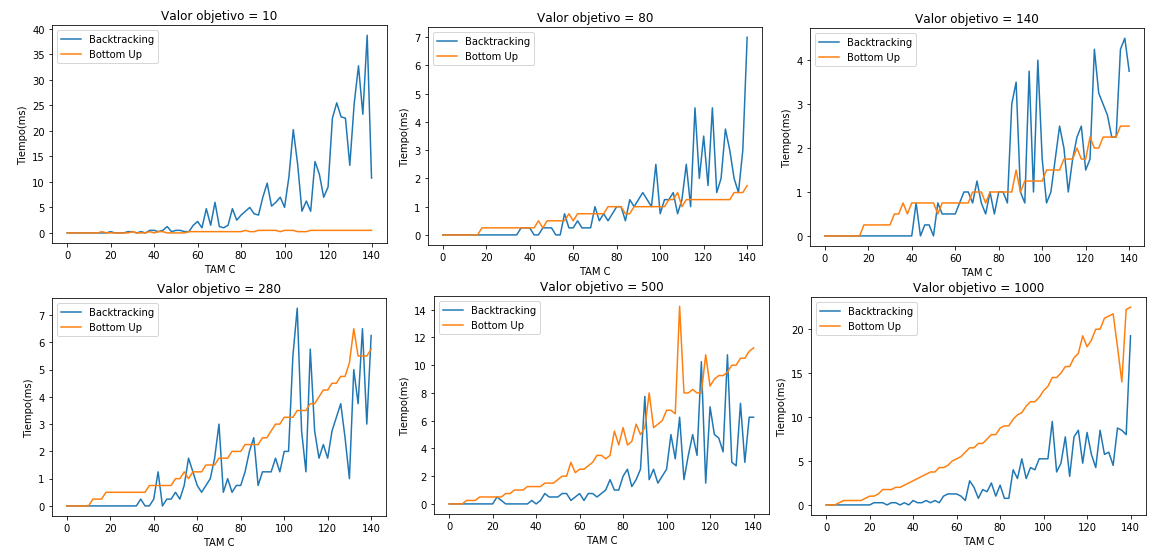
\includegraphics[scale=.6]{backvspd.png}
\begin{verse}
Es interesante ver la influencia del crecimiento de V para que la diferencia de performance empiece a igualarse y posteriormente a invertirse. Todavía más interesate si se mira con los anteriores gráficos, que se ve exactamente lo opuesto porque queríamos ver lo opuesto y que los dos grupos pueden verse como uno solo, en donde las diferentes etapas por las cuales los algoritmos se benefician o perjudican se hacen muy evidentes.\\
\end{verse}
%\begin{center}
%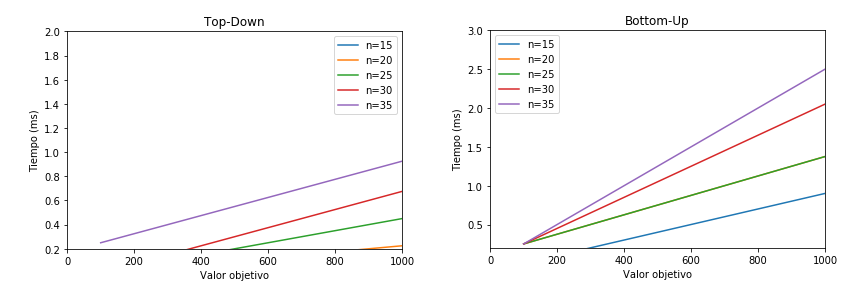
\includegraphics[scale=.8]{tdvsbu_lin.png}
%\end{center}

%\begin{center}
%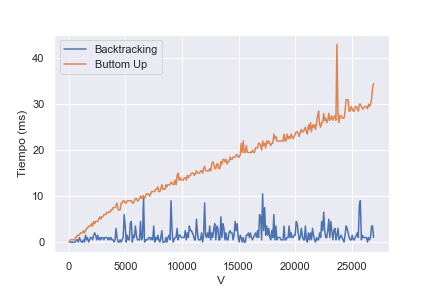
\includegraphics[scale=.4]{wc_bt_vs_bu_graph.png}\end{center}
%La explicación es simple: en estos casos particulares, backtracking actúa casi como un algoritmo lineal, porque son tantos los casos que evita calcular que es como si solo recorriera una vez a C, mientras que bottom up cada vez que V crece necesita matrices más grandes que recorrer.

%\subsection{Experimento 2}
%Ahora la cuestión es ver si existen instancias para las cuales convenga utilizar top-down en lugar de bottom up o backtracking. Para sacar ventaja frente a Bottom up necesitamos que n $\cdot$ V sea grande.
%Para lo siguiente construimos intanicias incrementando n y V simultaneamente, y los elementos de C generamos aleatoriamente de forma uniforme acotados por V.\\
%En el siguiente mapa de calor podemos ver de forma separada como es la relación de los tiempos de ejecución de cada algoritmo en función del tamaño de C y del valor objetivo. Como primer detalle vemos que las escalas de tiempo son diferentes: el top-down tiene gran parte de sus promedios de tiempos en los 5 segundos mientras que para el mismo tipo de instancias bottom up tiene promedios de 15. Por otro lado, vemos que en el bottom up los tiempos están más en función de n y V, es decir, es un algoritmo estable pero que se ve afectado por los tiempos que consume moverse en una matriz cada vez mas grande, a diferencia de top down. Este parece centraliza sus tiempos más grandes en una franja intermedia de los V. Por lo que venimos analizando, esto podría relacionarse con "peores" peores casos que al computarlos genera estas oscilaciones que venimos viendo, de modo que el top down ante casos en donde resuelve pocos subproblemas no se ve afectado por el n $\cdot$ V.

%Por último analicemos lo siguiente: Backtracking tiende a comportarse como lineal ante los casos en que V es de menor o igual orden que los elementos de C y bottom up demostró ser eficiente en ese tipo de instancias. La pregunta sería: si sabemos que estamos ante uno de estos contextos, cuál de los dos conviene?
%A simple viste se diría que backtracking, porque si es casi lineal claramente mejor que n x V. Sin embargo en nuestros análisis vimos que en los algoritmos recursivos las llamadas recursivas no son gratis y esto puede afectar la performance.
%\begin{center}
%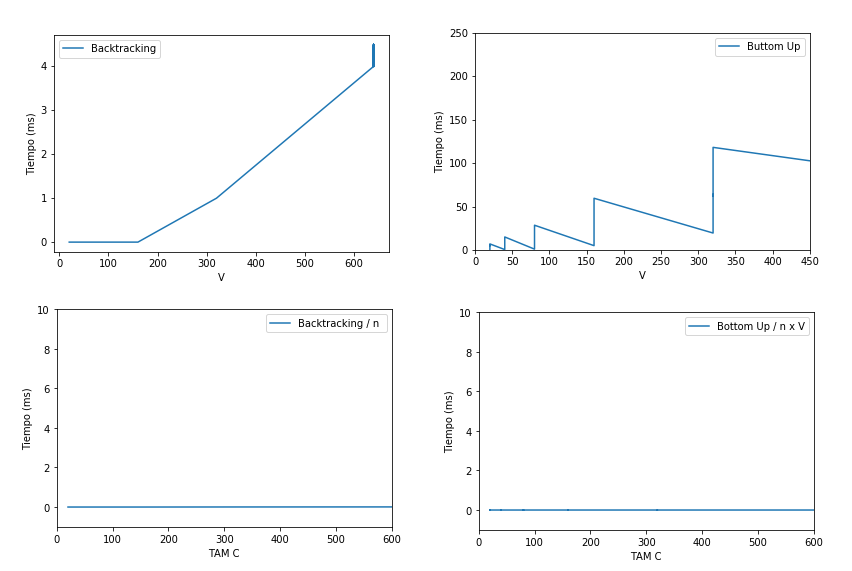
\includegraphics[scale=.4]{comp_bu_bt.png}
%\end{center}


%\subsection{Experimento 3}
%En la simulación de diferentes situaciones de la vida cotidiana se pueden utilizar distribuciones normales la generación de determinadas instancias. Sería interesante entonces analizar situaciones en las que los elementos estén generados de esta forma.
%Analicemos la siguiente, fijemos n en 15,20,25, que nuestros experimentos arrojaron que eran valores razonables para probar simultáneamente los algoritmos: si los elementos de C siguen una distribución normal de media n, el valor objetivo lo hacemos incrementarse hasta $n^{3}$ y la varianza = $\frac{n^{2}}{V}$ inicialmente y después varianza = $\frac{V}{n}$. En el primer caso es una instancia en donde a medida que crece V, los elementos de C sufren una menor dispersión. Esto puede indicar que, en Backtracking mientras V no sea de un orden mucho mayor a n, como los elementos van a estar cerca de V las podas van a tener mucho trabajo y el algoritmo será eficiente. Por otro lado, si la dispersión se incrementa con V, Backtracking va a empeorar su performance debido a su reducción en el uso de las podas.\\
%En el caso de Fuerza Bruta no se esperan cambios, dado que no importa la situación siempre hará lo mismo. Para Top-Down y Bottom Up, no se esperan grandes beneficios, de hecho para Top-Down es posible que cuando la dispersión sea alta se le generen lamadas recursivas muy pesadas y (por la alta densidad de los elementos) y empeore su performance.\\
%Se presentan los mapas de calor en función de V y n. En la parte superior están los gráficos cuando la dispersión disminuye cuando aumenta V.
%\begin{center}
%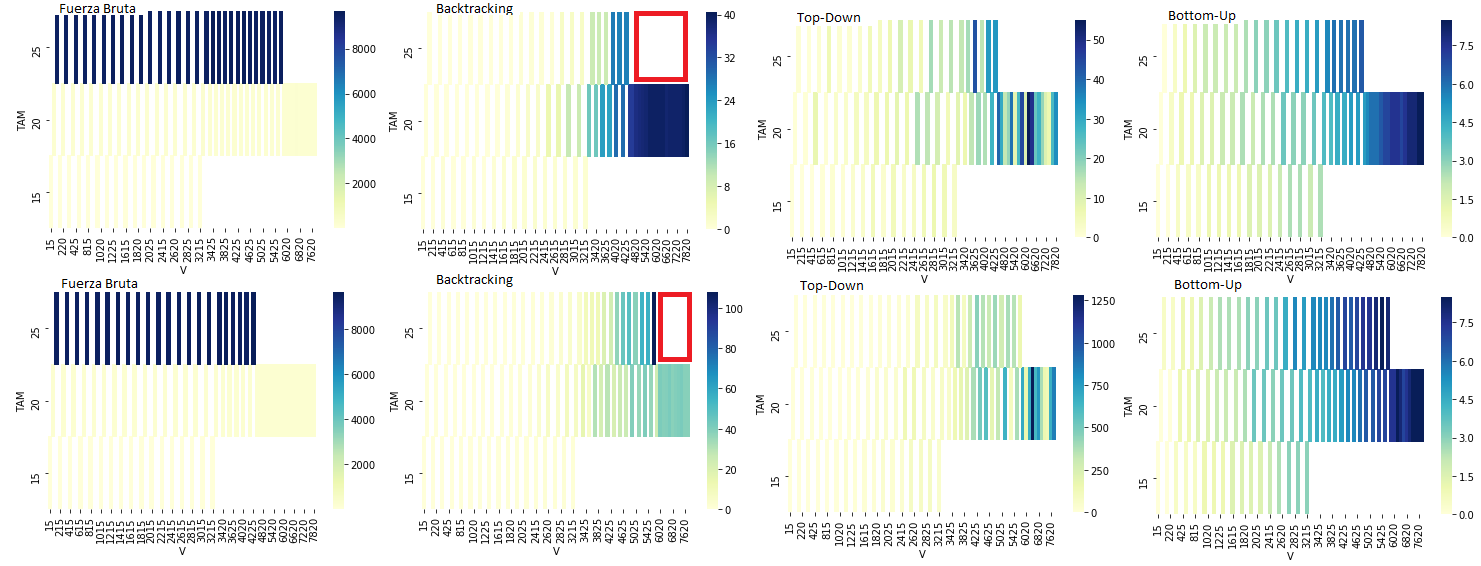
\includegraphics[scale=.4]{comp_distr_normal.png}
%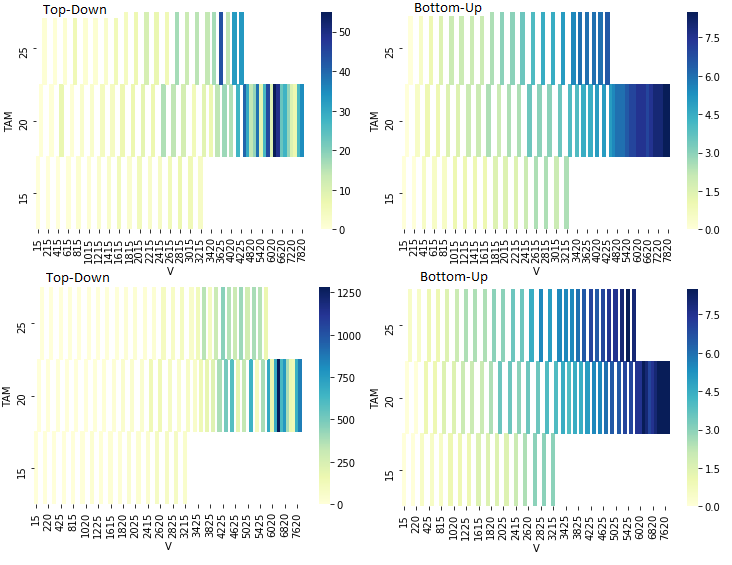
\includegraphics[scale=.5]{comp_distr_normal_2.png}
%\end{center}
\end{verse}
%Finalmente las ideas principales se puede apreciar que para Fuerza Bruta no hay cambios debido a que en cualquier caso realiza todos los subproblemas. Por otro lado Top-Down empeora considerablemente cuando la dispersión aumenta, aunque sorprende su alta eficiencia cuando es baja la dispersión. Lo que pasa es que no habíamos notado que Top-Down almacenará los resultados de los subproblemas y si esos subproblemas son muy parecidos (baja dispersión de los elementos) entonces se beneficiará mucho de esto, y esto evidentemente no se dará con una alta dispersión. \\
%Respecto de Backtracking hubo ciertas diferencias. Posiblemente se deba a que el hecho de que haya o no dispersión lo afecta en tanto y cuanto los elementos no se alejen mucho de V, porque en ese caso casi que actuará con un Fuerza Bruta. Como nota: marcas rojas indican que por temás de tiempo de procesamiento no se llegaron a completar.

\section{Conclusiones}

\begin{verse}
Durante la presentación de este trabajo se presentaron diferentes técnicas algorítmicas para hallar las soluciones del conocido problema {\it suma de subconjuntos}. Cada una de estás técnicas responden a diferentes formas de abordar el problema para llegar a una solución exacta y particularmente en nuestro caso la mejor. Inicialmente se hizo un análisis de la literatura del problema, mencionando diferentes algoritmos y sus objetivos principales. Posteriormente se escribieron cuatro diferentes algoritmos y desde ese momento se plantearon interrogantes acerca de qué tipo de situaciones o contextos podrían beneficiarlos. Finalmente se realizaron experimentos que permitieron conocer un poco más en profundidad los puntos débiles y fuertes de las soluciones, así como también adquirir la información suficiente a la hora de tomar decisiones de cuál de ellos experimentar en función del contexto, los recursos disponibles o las necesidades. \\
Los algoritmos que utilicen fuerza bruta quedan relegados para situaciones muy singulares, con tamaños de C muy pequeños, y su ventaja responde a la facilidad con la que se puede diseñar. Por el lado de Backtracking se puede encontraron situaciones en donde sería interesante aplicarlo. Estas se pueden englobar en las que los elementos de C son muy grandes respecto de V, y si V llegara a ser grande incluso vimos que le ganaría a los algoritmos de programación dinámica.
\\
Desde otro punto de las metodologías encontramos a Top-Down y Bottom up. Top Down fue un poco más rápido y también como era previsible, la performance de Bottom Up era directamente proporcional a los tamaños de n y V, y cuando estos eran muy grandes Top Down también lo padecía pero, como se vio en los mapas de calor, para muchas instancias al resolver sólo los subproblemas necesarios mejoraba mucho la performance respecto de Bottom Up. Este tipo de algoritmos son los mejores para resolver este problema cuando no se cumplen ciertas requerimientos como para aplicar Backtracking, porque no hay que olvidar que si C llegara a ser grande, con que una parte chica de los elementos no cumpla lo necesario, Backtracking ya es un algoritmo exponencial. Es decir, para utilizar esta técnica es necesario tener muy bien definido cómo serán V, |C| y los elementos de C para usarla. \\
\end{verse}

\section{Referencias}
\begin{verse}
$[3]$Dynamic training subset selection for supervised learning in Genetic Programming, Chris GathercolePeter Ross.\\
$[4]$Generalizing Cryptosystems Based on the Subset Sum Problem, Aniket Kate and Ian Goldberg\\
$[5]$Thomas Cormen, Algorithms and Optimization, Approximation Algorithms, pág 1106\\
$[6]$G. J. Woeginger, Exact Algorithms for NP-Hard Problems: A Survey, Lecture Notesin Computer Science 2570, pp. 185-207  \\
$[7]$Computing partitions with applications to the knapsack problem,  Journal of the Association for Computing Machinery\\
$[8]$Donald Knuth. \it{The Art Of Computer Programming : Fundamentals Algorithms}
\end{verse}
\section{Cambios}
\begin{enumerate}
\item Agregadas algunas cosas en la introducción.
\item La sección de Fuerza Bruta permaneció sin cambios.
\item Toda la sección de Backtracking fue modificada. Particularmente pseudocódigo, código fuente, justificación de complejidad, acorde a los cambios necesarios para llegar a la pedida. 
\item Se sacó el código fuente y se agrandaron los gráficos.
\item Agregados experimentos con escala logarítmica.
\item Modificadas algunas explicaciones de programación dinámica de complejidad. En Top-Down particularmente se modificó pseudocódigo y código fuente.
\item Modificados y agregados gran parte de los experimentos, para rehacerlos por las modificaciones de algunos algoritmos y en otros casos para agregar casos.
\item Agregados títulos ilustrativos en los experimentos.
\item Modificada las conclusiones a partir de los nuevos experimentos.
\item Se hace la entrega con las instancias que se usaron para testear y para experimentar.
\end{enumerate}

\end{document}
